
The system needs to be calibrated for the current installation height of the Kinect sensor. This is easily done in the Calibration Window, figure \ref{fig:Calibration}, which can be started under the \textit{System} tab in the menu bar. To the left is a thresholded depth image and to the right a histogram. The slider below the histogram adjusts the threshold level. The threshold should be set so that a "normal" person’s head and shoulders are left. Press Apply to save the changes. 

\begin{figure}[htb]
	\centering
	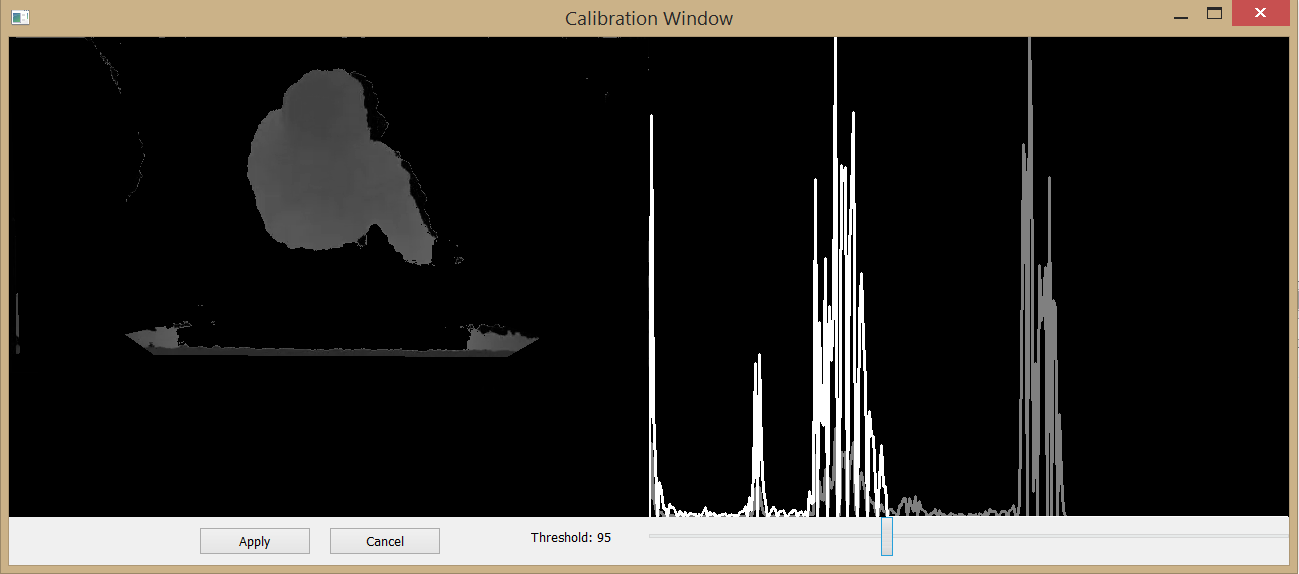
\includegraphics[width=\linewidth]{images/Calibration.png}
	\caption[Calibration Window]
	{\textit{Calibrating the depth threshold of the system. A histogram is shown to help the user. The adjusted histogram is shown in white and the raw histogram in gray.}}
	\label{fig:Calibration}  %Skapar referens till figuren
\end{figure}
